%% BioMed_Central_Tex_Template_v1.06
%%                                      %
%  bmc_article.tex            ver: 1.06 %
%                                       %

%%IMPORTANT: do not delete the first line of this template
%%It must be present to enable the BMC Submission system to
%%recognise this template!!

%%%%%%%%%%%%%%%%%%%%%%%%%%%%%%%%%%%%%%%%%
%%                                     %%
%%  LaTeX template for BioMed Central  %%
%%     journal article submissions     %%
%%                                     %%
%%          <8 June 2012>              %%
%%                                     %%
%%                                     %%
%%%%%%%%%%%%%%%%%%%%%%%%%%%%%%%%%%%%%%%%%


%%%%%%%%%%%%%%%%%%%%%%%%%%%%%%%%%%%%%%%%%%%%%%%%%%%%%%%%%%%%%%%%%%%%%
%%                                                                 %%
%% For instructions on how to fill out this Tex template           %%
%% document please refer to Readme.html and the instructions for   %%
%% authors page on the biomed central website                      %%
%% http://www.biomedcentral.com/info/authors/                      %%
%%                                                                 %%
%% Please do not use \input{...} to include other tex files.       %%
%% Submit your LaTeX manuscript as one .tex document.              %%
%%                                                                 %%
%% All additional figures and files should be attached             %%
%% separately and not embedded in the \TeX\ document itself.       %%
%%                                                                 %%
%% BioMed Central currently use the MikTex distribution of         %%
%% TeX for Windows) of TeX and LaTeX.  This is available from      %%
%% http://www.miktex.org                                           %%
%%                                                                 %%
%%%%%%%%%%%%%%%%%%%%%%%%%%%%%%%%%%%%%%%%%%%%%%%%%%%%%%%%%%%%%%%%%%%%%

%%% additional documentclass options:
%  [doublespacing]
%  [linenumbers]   - put the line numbers on margins

%%% loading packages, author definitions

%\documentclass[twocolumn]{bmcart}% uncomment this for twocolumn layout and comment line below
\documentclass{bmcart}

%%% Load packages
%\usepackage{amsthm,amsmath}
%\RequirePackage{natbib}
%\RequirePackage[authoryear]{natbib}% uncomment this for author-year bibliography
\RequirePackage{hyperref}
\usepackage[utf8]{inputenc} %unicode support
%\usepackage[applemac]{inputenc} %applemac support if unicode package fails
%\usepackage[latin1]{inputenc} %UNIX support if unicode package fails

% packages added by me
\usepackage{longtable}
\usepackage{float}
\usepackage{stfloats}
\usepackage{siunitx}
\sisetup{range-phrase = \text{--}}

%%%%%%%%%%%%%%%%%%%%%%%%%%%%%%%%%%%%%%%%%%%%%%%%%
%%                                             %%
%%  If you wish to display your graphics for   %%
%%  your own use using includegraphic or       %%
%%  includegraphics, then comment out the      %%
%%  following two lines of code.               %%
%%  NB: These line *must* be included when     %%
%%  submitting to BMC.                         %%
%%  All figure files must be submitted as      %%
%%  separate graphics through the BMC          %%
%%  submission process, not included in the    %%
%%  submitted article.                         %%
%%                                             %%
%%%%%%%%%%%%%%%%%%%%%%%%%%%%%%%%%%%%%%%%%%%%%%%%%

%% \def\includegraphic{}
%% \def\includegraphics{}

\usepackage{graphicx}
\graphicspath{{/Users/evayap/Documents/masters_thesis/ubcdiss_2/chapter3_figure/}{/Users/evayap/Documents/masters_thesis/ubcdiss_2/chapter2_figure/}{/Users/evayap/Documents/masters_thesis/ubcdiss_2/mm_figure/}{/Users/evayap/Documents/masters_thesis/ubcdiss_2/intro_figure/}}

%%% Put your definitions there:
\startlocaldefs
\endlocaldefs


%%% Begin ...
\begin{document}

%%% Start of article front matter
\begin{frontmatter}

\begin{fmbox}
\dochead{Research}

%%%%%%%%%%%%%%%%%%%%%%%%%%%%%%%%%%%%%%%%%%%%%%
%%                                          %%
%% Enter the title of your article here     %%
%%                                          %%
%%%%%%%%%%%%%%%%%%%%%%%%%%%%%%%%%%%%%%%%%%%%%%

\title{A sample article title}

%%%%%%%%%%%%%%%%%%%%%%%%%%%%%%%%%%%%%%%%%%%%%%
%%                                          %%
%% Enter the authors here                   %%
%%                                          %%
%% Specify information, if available,       %%
%% in the form:                             %%
%%   <key>={<id1>,<id2>}                    %%
%%   <key>=                                 %%
%% Comment or delete the keys which are     %%
%% not used. Repeat \author command as much %%
%% as required.                             %%
%%                                          %%
%%%%%%%%%%%%%%%%%%%%%%%%%%%%%%%%%%%%%%%%%%%%%%

\author[
   addressref={aff1},                   % id's of addresses, e.g. {aff1,aff2}
   corref={aff1},                       % id of corresponding address, if any
   noteref={n1},                        % id's of article notes, if any
   email={jane.e.doe@cambridge.co.uk}   % email address
]{\inits{JE}\fnm{Jane E} \snm{Doe}}
\author[
   addressref={aff1,aff2},
   email={john.RS.Smith@cambridge.co.uk}
]{\inits{JRS}\fnm{John RS} \snm{Smith}}

%%%%%%%%%%%%%%%%%%%%%%%%%%%%%%%%%%%%%%%%%%%%%%
%%                                          %%
%% Enter the authors' addresses here        %%
%%                                          %%
%% Repeat \address commands as much as      %%
%% required.                                %%
%%                                          %%
%%%%%%%%%%%%%%%%%%%%%%%%%%%%%%%%%%%%%%%%%%%%%%

\address[id=aff1]{%                           % unique id
  \orgname{Department of Zoology, Cambridge}, % university, etc
  \street{Waterloo Road},                     %
  %\postcode{}                                % post or zip code
  \city{London},                              % city
  \cny{UK}                                    % country
}
\address[id=aff2]{%
  \orgname{Marine Ecology Department, Institute of Marine Sciences Kiel},
  \street{D\"{u}sternbrooker Weg 20},
  \postcode{24105}
  \city{Kiel},
  \cny{Germany}
}

%%%%%%%%%%%%%%%%%%%%%%%%%%%%%%%%%%%%%%%%%%%%%%
%%                                          %%
%% Enter short notes here                   %%
%%                                          %%
%% Short notes will be after addresses      %%
%% on first page.                           %%
%%                                          %%
%%%%%%%%%%%%%%%%%%%%%%%%%%%%%%%%%%%%%%%%%%%%%%

\begin{artnotes}
%\note{Sample of title note}     % note to the article
\note[id=n1]{Equal contributor} % note, connected to author
\end{artnotes}

\end{fmbox}% comment this for two column layout

%%%%%%%%%%%%%%%%%%%%%%%%%%%%%%%%%%%%%%%%%%%%%%
%%                                          %%
%% The Abstract begins here                 %%
%%                                          %%
%% Please refer to the Instructions for     %%
%% authors on http://www.biomedcentral.com  %%
%% and include the section headings         %%
%% accordingly for your article type.       %%
%%                                          %%
%%%%%%%%%%%%%%%%%%%%%%%%%%%%%%%%%%%%%%%%%%%%%%

\begin{abstractbox}

\begin{abstract} % abstract
\parttitle{Background} %if any
Germline alterations have clinical implications for cancer patients and their families. Because the tumour genome contains both germline and somatic variants, clinical tumour sequencing presents an opportunity for pre-screening of germline variants. This framework is time- and cost-effective because only patients with potential germline variants are referred to downstream confirmatory testing. A key challenge in this framework is distinguishing between germline and somatic variants in the tumour. Tumour specimens are also commonly formalin-fixed paraffin-embedded (FFPE), which induces DNA damage that interferes with molecular testing. To determine the feasibility of leveraging tumour sequencing for identifying germline variants, the usability of FFPE DNA for germline testing must be evaluated and an approach to differentiate between germline and somatic variants must be established.

\parttitle{Methods} %if any

\parttitle{Results} %if any

\parttitle{Conclusions} %if any

\end{abstract}

%%%%%%%%%%%%%%%%%%%%%%%%%%%%%%%%%%%%%%%%%%%%%%
%%                                          %%
%% The keywords begin here                  %%
%%                                          %%
%% Put each keyword in separate \kwd{}.     %%
%%                                          %%
%%%%%%%%%%%%%%%%%%%%%%%%%%%%%%%%%%%%%%%%%%%%%%

\begin{keyword}
\kwd{Germline variants}
\kwd{Tumour-only sequencing}
\kwd{Formalin-fixed paraffin-embedded tumours}
\end{keyword}

% MSC classifications codes, if any
%\begin{keyword}[class=AMS]
%\kwd[Primary ]{}
%\kwd{}
%\kwd[; secondary ]{}
%\end{keyword}

\end{abstractbox}
%
%\end{fmbox}% uncomment this for twcolumn layout

\end{frontmatter}

%%%%%%%%%%%%%%%%%%%%%%%%%%%%%%%%%%%%%%%%%%%%%%
%%                                          %%
%% The Main Body begins here                %%
%%                                          %%
%% Please refer to the instructions for     %%
%% authors on:                              %%
%% http://www.biomedcentral.com/info/authors%%
%% and include the section headings         %%
%% accordingly for your article type.       %%
%%                                          %%
%% See the Results and Discussion section   %%
%% for details on how to create sub-sections%%
%%                                          %%
%% use \cite{...} to cite references        %%
%%  \cite{koon} and                         %%
%%  \cite{oreg,khar,zvai,xjon,schn,pond}    %%
%%  \nocite{smith,marg,hunn,advi,koha,mouse}%%
%%                                          %%
%%%%%%%%%%%%%%%%%%%%%%%%%%%%%%%%%%%%%%%%%%%%%%

%%%%%%%%%%%%%%%%%%%%%%%%% start of article main body
% <put your article body there>

%%%%%%%%%%%%%%%%%%%%%%%%%%%%%%%%%%%%%%%%%%%%%%
\section*{Background}
%%%%%%%%%%%%%%%%%%%%%%%%%%%%%%%%%%%%%%%%%%%%%%

Germline alterations have clinical implications for cancer patients and their families. Inherited predisposition to cancer can be predicted

Tumour sequencing has been rapidly integrated into clinical oncology Because the tumour genome contains both germline and somatic variants, clinical tumour sequencing presents an opportunity for pre-screening of germline variants. This framework is time- and cost-effective because only patients with potential germline variants would be referred to follow-up germline testing. Follow-up germline testing could A key challenge in this framework is distinguishing between germline and somatic variants in the tumour.

Tumour specimens are also commonly formalin-fixed paraffin-embedded (FFPE), which induces DNA damage that interferes with molecular testing.

Genomic analyses of tumours can not only reveal actionable somatic mutations, but also germline variants with clinical implications for patients and their families. Thus, clinical tumour sequencing presents an opportunity to perform initial screening for germline variants. This framework is cost-saving because only patients with potential germline variants would be referred to downstream confirmatory testing.

%%%%%%%%%%%%%%%%%%%%%%%%%%%%%%%%%%%%%%%%%%%%%%
\section*{Methods}
%%%%%%%%%%%%%%%%%%%%%%%%%%%%%%%%%%%%%%%%%%%%%%

\subsection*{Patient samples}

Blood and FFPE tumour samples were acquired from 213 patients who provided informed consent for The OncoPanel Pilot (TOP) study (Human Research Ethics Protocol H14­-01212), a pilot study to optimize the OncoPanel, which is an amplicon-based targeted NGS panel for solid tumours. The TOP study also assessed the OncoPanel's application for guiding disease management and therapeutic intervention. One blood sample and four FFPE tumours were sequenced in duplicates, which resulted in 217 tumour-normal paired samples (434 sequencing libraries were included in our analyses). Patients in the TOP study were those with advanced cancers including CRC, lung cancer, melanoma, gastrointestinal stromal tumour (GIST), and other cancers (\autoref{cancertypes}). The age of paraffin block for tumour samples ranged from 18 to 5356 days with a median of 274 days.

\subsection*{Sample preparation, library construction, and Illumina sequencing}
Genomic DNA was extracted from blood and FFPE tumour samples using the Gentra Autopure LS DNA preparation platform and QIAamp DNA FFPE tissue kit (Qiagen, Hilden, Germany), respectively. The extracted DNA was sheared according to a previously described protocol \cite{Bosdet2013} to obtain approximate sizes of 3 Kb followed by PCR primer merging, amplification of target regions, and adapter ligation using the Thunderstorm NGS Targeted Enrichment System (RainDance Technologies, Lexington, MA) as per manufacturer's protocol. Barcoded amplicons were sequenced with the Illumina MiSeq system for paired end sequencing with a v2 250-bp kit (Illumina, San Diego, CA).

\subsection*{OncoPanel (Amplicon-based targeted sequencing panel for solid tumours)}

The OncoPanel assesses coding exons and clinically relevant hotspots of 15 cancer-related genes and six PGx genes. Germline alterations in the six PGx genes could serve as predictors of susceptibility to chemotherapy-induced toxicity. Primers were designed by RainDance Technologies (Lexington, MA) using the GRCh37/hg19 human reference genome to generate 416 amplicons between 56 bp and 288 bp in size, which interrogate $\sim$ 20 Kb of target bases. Complete list of genes and gene reference models for the OncoPanel as well as target regions and amplicons are presented in Supplemental Materials.

\subsection*{Variant calling pipeline}

\subsubsection*{Read alignment and variant calling}

Reads that passed the Illumina Chastity filter were aligned to the hg19 human reference genome using the BWA mem algorithm (version 0.5.9) with default parameters, and the alignments were processed and converted to the BAM format using SAMtools (version 0.1.18). The SAMtools \texttt{mpileup} function \texttt{(samtools mpileup -BA -d 500000 -L 500000 -q 1)} was used to generate pileup files for all target bases followed by variant calling with the VarScan2 \texttt{mpileup2cns} (version 2.3.6) function with parameter thresholds of VAF $\geq$ 0.1 and Phred-scaled BAQ score $\geq$ 20 \texttt{(--min-var-freq 0.1 --min-avg-qual 20 --strand-filter 0 --p-value 0.01 --output-vcf --variants)}.

\subsubsection*{Identifying patients with homozygous minor alleles that are present the hg19 reference genome}

Four genomic positions at which the hg19 human reference genome contained the minor alleles were identified (\autoref{potential_risk_alleles}). Hence, patients homozygous for these four minor alleles would not be identified by our standard variant calling procedure. For these four genomic sites, our method for variant calling was modified to provide calls for every patient in the cohort. The VarScan2 \texttt{mpileup2cns} function was used with parameter thresholds of VAF $\geq$ 0.25, VAF to call homozygote $\geq$ 0.9, BAQ score $\geq$ 20, and fraction of variant reads from each strand $\geq$ 0.1 \texttt{(--min-var-freq 0.25 --min-freq-for-hom 0.9 --min-avg-qual 20 --strand-filter 1 --p-value 0.01 --output-vcf)}. Next, allelic statuses were re-assigned, in which wild type calls were re-assigned as homozygous variants, while homozygous variants were re-assigned as wild type calls. Corrections to the VAFs of these four genomic sites were also made to ensure that the VAFs reflected percentage of reads with the minor alleles.

\subsubsection*{Variant filtering}

Variant calls were filtered using the VarScan2 \texttt{fpfilter} function with fraction of variant reads from each strand $\geq$ 0.1 and default thresholds for other parameters (\autoref{varscan_fpfilter_parameters}). The VarScan2 \texttt{fpfilter} removed 247 low quality variants. Seventy germline variants in the blood were also excluded from our analysis because these variants in the tumours were filtered by the VarScan2 \texttt{fpfilter}. There were also 16 risk allele calls in tumour samples that did not pass the strand filter, causing the removal of 10 risk allele calls in the blood samples from our evaluation. Overall, a total of 343 calls were excluded by the VarScan2 \texttt{fpfilter} and strand filter. Manual inspection was performed for a subset of variants, including variants detected within primer regions and in PGx genes, using the Integrative Genomics Viewer (IGV, version 2.3). This resulted in the removal of 500 spurious calls, which stemmed from software bugs, sequencing artifacts, primer masking, and primer artifacts (\autoref{spurious_calls}). Eleven low coverage calls ($\leq$ 100x) were also excluded from our analysis. Implementation of this filtering pipeline reduced the raw variant output of 5288 calls from 217 paired tumour-blood samples (434 sequencing libraries) to 4434 calls (\autoref{variant_pipeline}B).

\subsubsection*{Variant annotation and interpretation}

SnpEff (version 4.2) was used for effect prediction, and the SnpSift package in SnpEff was used to annotate variants with databases such as dbSNP (b138), COSMIC (version 70), 1000 Genomes Project, and ExAC (release 0.3) for interpretation. Clinical significance reported by the ClinVar database and literature review were also used for variant interpretation.

\subsection*{Sequence analysis}

A custom Python script was used to process BAM files to quantify the number of on-target aligned (reads that map to target regions), off-target aligned (reads that map to hg19 but not target regions), and unaligned reads with a Phred-scaled mapping quality (MAPQ) score $\geq$ 10. Unaligned reads were also screened against microbial sequences, including viruses, archaea, bacteria, and fungi, to ensure that samples did not contain significant amount of microbial contaminants. Coverage depth for target bases with MAPQ $\geq$ 1 and BAQ $\geq$ 20 were obtained using bam-readcount (https://github.com/genome/bam-readcount). To measure coverage depth of amplicons, the SAMtools \texttt{view} function was used to filter for reads with MAPQ $\geq$ 1 \texttt{(samtools view -b -q 1)} followed by the bedtools \texttt{intersect} function (version 2.25.0) to quantify the number of reads that overlap with amplicon positions \texttt{(intersect -a \$AMPLICON\_POSITIONS -b \$BAM\_FILE -f 0.85 -r -c)}.

Per-base metrics generated using bam-readcount were also used for assessment of sequence artifacts. A custom R script was used to count and categorize the different groups of base changes (i.e. C$>$T/G$>$A, A$>$G/T$>$C, C$>$A/G$>$T, A$>$C/T$>$G, C$>$G/G$>$C, and A$>$T/T$>$A). Unless stated otherwise, analysis of sequence artifacts excluded true variants identified by our VarScan2 variant calling pipeline and base changes with VAF $<$ 1\%, which were considered sequencing errors. All statistical analyses and data visualization were performed using the R statistical software package (version 3.3.2) and associated open source packages.

%%%%%%%%%%%%%%%%%%%%%%%%%%%%%%%%%%%%%%%%%%%%%%%%%%%%%%%%%%%%%%%%%%%%%%
\subsection*{Application of VAF thresholds to separate germline alterations from somatic mutations}

Variants in the tumours that passed our filtering criteria were subjected to VAF thresholds between 10--45\%. At each VAF cut-off, variants that were not filtered out were considered predicted germline variants. Given that all tumour samples have matched blood samples, true positives were identified as predicted germline variants that overlap with variants in the blood. Conversely, false negatives were identified as variants that were filtered out by the VAF cut-off (predicted as somatic), but were present in the blood samples. Sensitivity at each VAF threshold was calculated by dividing the number of true positives with the sum of true positives and false negatives. Because predicted germline variants would be referred to follow-up germline testing, positive predictive values (PPVs) were calculated at each VAF cut-off to evaluate precision of our approach. False positives were identified as predicted germline variants that were absent in the blood, and PPV was calculated by dividing the number of true positives with the sum of true positives and false positives.

%%%%%%%%%%%%%%%%%%%%%%%%%%%%%%%%%%%%%%%%%%%%%%
\section*{Results}
%%%%%%%%%%%%%%%%%%%%%%%%%%%%%%%%%%%%%%%%%%%%%%

\subsection*{Comparison of efficiency in amplicon enrichment and sequencing results between blood and FFPE specimens}

To determine whether FFPE DNA is viable for identifying germline variants, we characterized the effect of formalin-induced DNA damage on efficiency in amplicon enrichment and sequencing metrics. We compared these outcomes to DNA isolated from blood, which is a gold standard for germline testing. Efficiency in amplicon enrichment was measured as the log\textsubscript{2} fold change between DNA input and amplicon yield (log\textsubscript{2} (Amplicon Yield/DNA Input)) and compared between FFPE specimens to blood. There was a significant decrease in enrichment efficiency in FFPE specimens compared to blood (Wilcoxon signed-rank test, \textit{W} = 24754, \textit{Z} = 12.7, \textit{p} = \num{4.6e-57}, \textit{r} = 0.61; \autoref{dna_input_amp_yield}). The median log\textsubscript{2} (Amplicon Yield/DNA Input) for blood was 1.04, whereas the median log\textsubscript{2} (Amplicon Yield/DNA Input) for FFPE specimens was -0.332. This demonstrates that production of amplicons was less efficient in FFPE specimens compared to blood.

We also compared read alignments between FFPE specimens and blood.

\subsection*{Reduced coverage depth in FFPE specimens is more pronounced for longer amplicons}

\subsection*{Deamination effects lead to increased C$>$T/G$>$A transitions in FFPE specimens}

\subsection*{Increased age of paraffin block results in reduced amplicon yield and elevated level of C$>$T/G$>$A sequence artifacts}

\subsection*{Frequency and interpretation of germline alterations in patients from TOP cohort}

\subsection*{The majority of germline alterations in the blood are retained in the tumour}

\subsection*{Application of VAF thresholds to separate germline alterations from somatic mutations in tumour-only analyses}

%%%%%%%%%%%%%%%%%%%%%%%%%%%%%%%%%%%%%%%%%%%%%%
\section*{Discussion}
%%%%%%%%%%%%%%%%%%%%%%%%%%%%%%%%%%%%%%%%%%%%%%

%
Thus we observe that this expected value is finite for all $v>0$ (also see \cite{koon,khar,zvai,xjon,marg}).
%\nocite{oreg,schn,pond,smith,marg,hunn,advi,koha,mouse}

%%%%%%%%%%%%%%%%%%%%%%%%%%%%%%%%%%%%%%%%%%%%%%
%%                                          %%
%% Backmatter begins here                   %%
%%                                          %%
%%%%%%%%%%%%%%%%%%%%%%%%%%%%%%%%%%%%%%%%%%%%%%

\begin{backmatter}

\section*{Competing interests}
  The authors declare that they have no competing interests.

\section*{Author's contributions}
    Text for this section \ldots

\section*{Acknowledgements}
  Text for this section \ldots
%%%%%%%%%%%%%%%%%%%%%%%%%%%%%%%%%%%%%%%%%%%%%%%%%%%%%%%%%%%%%
%%                  The Bibliography                       %%
%%                                                         %%
%%  Bmc_mathpys.bst  will be used to                       %%
%%  create a .BBL file for submission.                     %%
%%  After submission of the .TEX file,                     %%
%%  you will be prompted to submit your .BBL file.         %%
%%                                                         %%
%%                                                         %%
%%  Note that the displayed Bibliography will not          %%
%%  necessarily be rendered by Latex exactly as specified  %%
%%  in the online Instructions for Authors.                %%
%%                                                         %%
%%%%%%%%%%%%%%%%%%%%%%%%%%%%%%%%%%%%%%%%%%%%%%%%%%%%%%%%%%%%%

% if your bibliography is in bibtex format, use those commands:
\bibliographystyle{bmc-mathphys} % Style BST file (bmc-mathphys, vancouver, spbasic).
\bibliography{bmc_article}      % Bibliography file (usually '*.bib' )
% for author-year bibliography (bmc-mathphys or spbasic)
% a) write to bib file (bmc-mathphys only)
% @settings{label, options="nameyear"}
% b) uncomment next line
%\nocite{label}

% or include bibliography directly:
% \begin{thebibliography}
% \bibitem{b1}
% \end{thebibliography}

%%%%%%%%%%%%%%%%%%%%%%%%%%%%%%%%%%%
%%                               %%
%% Figures                       %%
%%                               %%
%% NB: this is for captions and  %%
%% Titles. All graphics must be  %%
%% submitted separately and NOT  %%
%% included in the Tex document  %%
%%                               %%
%%%%%%%%%%%%%%%%%%%%%%%%%%%%%%%%%%%

%%
%% Do not use \listoffigures as most will included as separate files

\newpage
\section*{Figures}

%%%%%%%%%%%%%%%%%%%%%%%%%%%%%%%%%%%%%%%%%%%%%%%%%%%%%%%%%%%%%%%%%%%%%%
\begin{figure}[h!]
\centering
	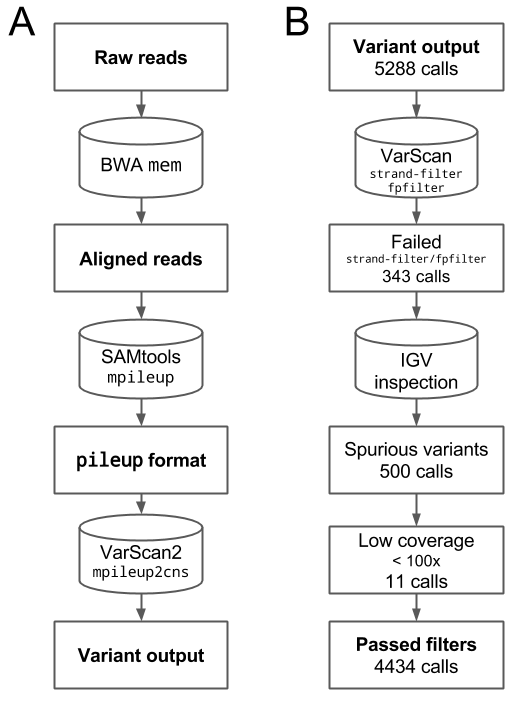
\includegraphics[scale=0.4]{variant_pipeline3.png}
	\caption{Pipelines for (A) variant calling and (B) filtering.}
	\label{variant_pipeline}
\end{figure}

%%%%%%%%%%%%%%%%%%%%%%%%%%%%%%%%%%%%%%%%%%%%%%%%%%%%%%%%%%%%%%%%%%%%%%
\begin{figure}[h!]
  \caption{\csentence{Sample figure title.}
      Figure legend text.}
      \end{figure}

%%%%%%%%%%%%%%%%%%%%%%%%%%%%%%%%%%%%%%%%%%%%%%%%%%%%%%%%%%%%%%%%%%%%%%

%%%%%%%%%%%%%%%%%%%%%%%%%%%%%%%%%%%
%%                               %%
%% Tables                        %%
%%                               %%
%%%%%%%%%%%%%%%%%%%%%%%%%%%%%%%%%%%


%% Use of \listoftables is discouraged.
%%
\section*{Tables}

%%%%%%%%%%%%%%%%%%%%%%%%%%%%%%%%%%%%%%%%%%%%%%%%%%%%%%%%%%%%%%%%%%%%%%
\begin{table}[H]
\caption{Distribution of cancer types in the TOP cohort.}
\label{cancertypes}
\centering
      \begin{tabular}{lccc}
        \hline
        Cancer Type & Number of Cases & Percentage (\%) \\ \hline
        Colorectal & 97 & 46 \\
        Lung & 60 & 28 \\
        Melanoma & 18 & 8 \\
				Other\textsuperscript{$\dagger$} & 16 & 8 \\
				GIST & 7 & 3 \\
				Sarcoma & 4 & 2 \\
				Neuroendocrine & 4 & 2 \\
				Cervical & 2 & 0.9 \\
				Ovarian & 2 & 0.9 \\
				Breast & 2 & 0.9 \\
				Unknown & 1 & 0.5 \\ \hline
      \end{tabular} \\
			\vspace{0.3cm}
\raggedright
\textsuperscript{$\dagger$}This category includes thyroid, peritoneum, Fallopian tube, gastric, endometrial, squamous cell carcinoma, anal, salivary gland, peritoneal epithelial mesothelioma, adenoid cystic carcinoma, pancreas, breast, gall bladder, parotid epithelial myoepithelial carcinoma, carcinoid, and small bowel cancers.
\end{table}

%%%%%%%%%%%%%%%%%%%%%%%%%%%%%%%%%%%%%%%%%%%%%%%%%%%%%%%%%%%%%%%%%%%%%%
\begin{table}[H]
    \caption{Gene reference models for HGVS nomenclature of OncoPanel genes.}
    \label{tbl:genemodel}
    \centering
    \begin{tabular}{llll}
    \hline
    Gene & Protein & Reference Model \\
    \hline
    \multicolumn{3}{l}{\textit{Cancer-related}}
    \\
    AKT1 & Protein kinase B & NM\_001014431.1 \\
    ALK & Anaplastic lymphoma receptor tyrosine kinase & NM\_004304.3 \\
    BRAF & Serine/threonine-protein kinase B-Raf & NM\_004333.4 \\
    EGFR & Epidermal growth factor receptor & NM\_005228.3 \\
    HRAS & GTPase HRas & NM\_005343.2 \\
    MAPK1 & Mitogen-activated protein kinase 1 & NM\_002745.4 \\
    MAP2K1 & Mitogen-activated protein kinase kinase 1 & NM\_002755.3 \\
    MTOR & Serine/threonine-protein kinase mTOR & NM\_004958.3 \\
    NRAS & Neuroblastoma RAS viral oncogene homolog & NM\_002524.3 \\
    PDGFRA & Platelet-derived growth factor receptor alpha & NM\_006206.4 \\
    PIK3CA & Phosphatidylinositol-4,5-bisphosphate 3-kinase catalytic subunit alpha & NM\_006218.2 \\
    PTEN & Phosphatase and tensin homolog & NM\_000314.4 \\
    STAT1 & Signal transducer and activator of transcription 1 & NM\_007315.3 \\
    STAT3 & Signal transducer and activator of transcription 3 & NM\_139276.2 \\
    TP53 & Tumor protein P53 & NM\_000546.5 \\
    \\
    \multicolumn{3}{l}{\textit{Pharmacogenomic-related}}
    \\
    DPYD & Dihydropyrimidine dehydrogenase & NM\_000110.3 \\
    GSTP1 & Glutathione S-rransferase pi 1 & NM\_000852.3 \\
    MTHFR & Methylenetetrahydrofolate reductase & NM\_005957.4 \\
    TYMP & Thymidine phosphorylase & NM\_001113755.2 \\
    TYMS & Thymidylate synthetase & NM\_001071.2 \\
    UGT1A1 & Uridine diphosphate (UDP)-glucuronosyl transferase 1A1 & NM\_000463.2\\
    \hline
    \end{tabular}
\end{table}

%%%%%%%%%%%%%%%%%%%%%%%%%%%%%%%%%%%%%%%%%%%%%%%%%%%%%%%%%%%%%%%%%%%%%%
\begin{longtable}{p{0.08\linewidth}|p{0.05\linewidth}p{0.1\linewidth}p{0.13\linewidth}p{0.16\linewidth}p{0.2\linewidth}}
    \caption{Potential minor alleles in the hg19 human reference genome within the target regions of the OncoPanel. (Supplementary)}
    \label{potential_risk_alleles}
        \\
        \hline
        Gene & Chr & Pos & Minor Allele & dbSNP ID & HGVS\textsuperscript{*}
				\\
				\hline
        DPYD & chr1 & 98348885 & C & rs1801265 & p.Cys29Arg c.85T$>$C
        \\
        MTOR & chr1 & 11205058 & G & rs386514433; rs1057079 & p.Ala1577Ala c.4731A$>$G
        \\
        & chr1 & 11288758 & C & rs1064261 & p.Asn999Asn c.2997T$>$C
        \\
        TP53 & chr17 & 7579472 & C & rs1042522 & p.Arg72Pro c.215G$>$C
        \\
				\hline
        \caption*{\textsuperscript{*}Description of sequence variants according to the HGVS recommendations.}
\end{longtable}

%%%%%%%%%%%%%%%%%%%%%%%%%%%%%%%%%%%%%%%%%%%%%%%%%%%%%%%%%%%%%%%%%%%%%%
\begin{table}[H]
\caption{Thresholds for parameters of VarScan2 \texttt{fpfilter} used for filtering raw variant output. (Supplementary)}
\label{varscan_fpfilter_parameters}
\centering
      \begin{tabular}{p{0.3\linewidth}p{0.56\linewidth}cp{0.1\linewidth}}
        \hline
        Parameter & Description & Threshold
				\\
				\hline
				\texttt{--min-var-count} & Min number of var-supporting reads & 4
				\\
        \texttt{--min-var-count-lc} & Min number of var-supporting reads when depth below somaticPdepth & 2
        \\
        \texttt{--min-var-freq} & Min variant allele frequency & 0.1
				\\
        \texttt{--max-somatic-p} & Max somatic p-value & 0.05
				\\
        \texttt{--max-somatic-p-depth} & Depth required to test max somatic p-value & 10
				\\
        \texttt{--min-ref-readpos} & Min average read position of ref-supporting reads & 0.1
				\\
        \texttt{--min-var-readpos} & Min average read position of var-supporting reads & 0.1
				\\
        \texttt{--min-ref-dist3} & Min average distance to effective 3' end of ref reads & 0.1
				\\
        \texttt{--min-var-dist3} & Min average distance to effective 3' end of variant reads & 0.1
				\\
        \texttt{--min-strandedness} & Min fraction of variant reads from each strand & 0.1
				\\
        \texttt{--min-strand-reads} & Min allele depth required to perform the strand tests & 5
				\\
        \texttt{--min-ref-basequal} & Min average base quality for ref allele & 15
				\\
        \texttt{--min-var-basequal} & Min average base quality for var allele & 15
				\\
        \texttt{--min-ref-avgrl} & Min average trimmed read length for ref allele & 90
				\\
        \texttt{--min-var-avgrl} & Min average trimmed read length for var allele & 90
        \\
        \texttt{--max-rl-diff} & Max average relative read length difference (ref - var) & 0.25
        \\
        \texttt{--max-ref-mmqs} & Max mismatch quality sum of ref-supporting reads & 100
        \\
        \texttt{--max-var-mmqs} & Max mismatch quality sum of var-supporting reads & 100
        \\
        \texttt{--max-mmqs-diff} & Max average mismatch quality sum (var - ref) & 50
        \\
        \texttt{--min-ref-mapqual} & Min average mapping quality for ref allele & 15
        \\
        \texttt{--min-var-mapqual} & Min average mapping quality for var allele & 15
        \\
        \texttt{--max-mapqual-diff} & Max average mapping quality (ref - var) & 50
        \\
				\hline
      \end{tabular}
\end{table}

%%%%%%%%%%%%%%%%%%%%%%%%%%%%%%%%%%%%%%%%%%%%%%%%%%%%%%%%%%%%%%%%%%%%%%
\begin{longtable}{p{0.08\linewidth}p{0.05\linewidth}p{0.1\linewidth}p{0.04\linewidth}p{0.04\linewidth}p{0.4\linewidth}}
    \caption{Spurious variants removed by the variant filtering pipeline. (Supplementary)}
    \label{spurious_calls}
        \\
        \hline
        Gene & Chr & Pos & Ref & Alt & Reason
				\\
				\hline
				KIT & chr4 & 55599268 & C & T & Variant masked by primer in FFPE specimen
				\\
        MAPK1 & chr22 & 22162126 & A & G & Variant masked by primer in FFPE specimen
        \\
        MTOR & chr1 & 11186783 & G & A & Sequencing artifact within primer region
        \\
        MTOR & chr1 & 11190646 & G & A & Variant masked by primer in FFPE specimen
        \\
        TYMP & chr22 & 50964446 & A & T & Poor target region, alignment of different sized amplicons
        \\
        TYMP & chr22 & 50964862 & A & T & Poor target region, alignment of different sized amplicons
        \\
        TYMS & chr18 & 673449 & G & C & VarScan2 bug after chr18:673443 c.*447\_*452delTTAAAG
        \\
        UGT1A1 & chr2 & 234668879 & CAT & C & Sequencing artifact at AT repeats in promoter
        \\
        UGT1A1 & chr2 & 234668881 & T & TAC & VarScan2 bug after AT insertion in promoter
        \\
				\hline
\end{longtable}

%%%%%%%%%%%%%%%%%%%%%%%%%%%%%%%%%%%%%%%%%%%%%%%%%%%%%%%%%%%%%%%%%%%%%%
\begin{table}[H]
\caption[Multiple linear regression to predict log\textsubscript{2} fold change between amplicon coverage depth in blood and FFPE specimens based on amplicon length and GC content.]{Multiple linear regression to predict log\textsubscript{2} fold change between amplicon coverage depth in blood and FFPE specimens (\mbox{log\textsubscript{2} (Median Coverage\textsubscript{FFPE}/Median Coverage\textsubscript{Blood})}) based on amplicon length and GC content.}
\label{tbl:multiple_regression}
\centering
      \begin{tabular}{l|ccccl}
        Variable & Unstandardized Coefficient & Standard Error & Standardized Coefficient & \textit{p}-value
        \\
        \hline
        Length (bp) & \num{-6.97e-3} & \num{2.59e-4} & \num{-7.56e-1} & \num{7.45e-93}
				\\
				GC Content (\%) & \num{-1.03e-2} & \num{1.01e-3} & \num{-2.88e-1} & \num{4.71e-22}
				\\
				\hline
				\\
				 & \multicolumn{4}{r}{Intercept = 1.63, Adjusted R\textsuperscript{2} = 0.673}
				\\
				 & \multicolumn{4}{r}{\textit{F}(2, 413) = 427.6, \textit{p}-value = \num{2.41e-101}}
				\\
				\hline
      \end{tabular} \\
\end{table}

%%%%%%%%%%%%%%%%%%%%%%%%%%%%%%%%%%%
%%                               %%
%% Additional Files              %%
%%                               %%
%%%%%%%%%%%%%%%%%%%%%%%%%%%%%%%%%%%

\section*{Additional Files}
  \subsection*{Additional file 1 --- Sample additional file title}
    Additional file descriptions text (including details of how to
    view the file, if it is in a non-standard format or the file extension).  This might
    refer to a multi-page table or a figure.

  \subsection*{Additional file 2 --- Sample additional file title}
    Additional file descriptions text.


\end{backmatter}
\end{document}
